% Adjust these for the path of the theme and its graphics, relative to this file
%\usepackage{beamerthemeFalmouthGamesAcademy}
\usepackage{../../beamerthemeFalmouthGamesAcademy}
\usepackage{multimedia}
\graphicspath{ {../../} }

% Default language for code listings
\lstset{language=C++,
        morekeywords={each,in,nullptr}
}

% For strikethrough effect
\usepackage[normalem]{ulem}
\usepackage{wasysym}

\usepackage{algpseudocode}

\usepackage{pdfpages}

\usepackage{fancyvrb}

% http://www.texample.net/tikz/examples/state-machine/
\usetikzlibrary{arrows,automata}

\setbeamertemplate{navigation symbols}{}

\newcommand{\modulecode}{COMP260}\newcommand{\moduletitle}{Distributed Systems}\newcommand{\sessionnumber}{5}

\begin{document}
\title{\sessionnumber: Module Induction}
\subtitle{\modulecode: \moduletitle}

\frame{\titlepage} 

\begin{frame}
	\frametitle{Learning Outcomes}
	\begin{itemize}
		\item \textbf{Explain} the aims and expectations of the final year project
		\item \textbf{Propose} appropriate methodologies to conduct scholarly research
		\item \textbf{Recall} Falmouth University's policy on research ethics and the procedure for obtaining ethics approval
	\end{itemize}
\end{frame}

\part{Assignments}
\frame{\partpage}

\begin{frame}{COMP250 assignments}
	\pause Similar to COMP220:
	\begin{itemize}
		\pause\item Portfolio task (90\%)
		\pause\item Research journal (10\%)
	\end{itemize}
\end{frame}

\begin{frame}{COMP250 portfolio task}
	\begin{itemize}
		\pause\item Assignment brief on LearningSpace
		\pause\item Basically, develop an \textbf{AI component} for a game
		\pause\item In the next two weeks:
			\begin{itemize}
				\pause\item Prepare a \textbf{proposal}
				\pause\item Start \textbf{collecting} and \textbf{reading} appropriate literature
			\end{itemize}
		\pause\item For the rest of today: begin preparing your \textbf{proposal}
		\pause\item Not sure what's technically feasible? \textbf{Ask me!}
	\end{itemize}
\end{frame}


\part{Ethics of analytics}
\frame{\partpage}

\begin{frame}
	\begin{columns}
		\begin{column}{0.48\textwidth}
			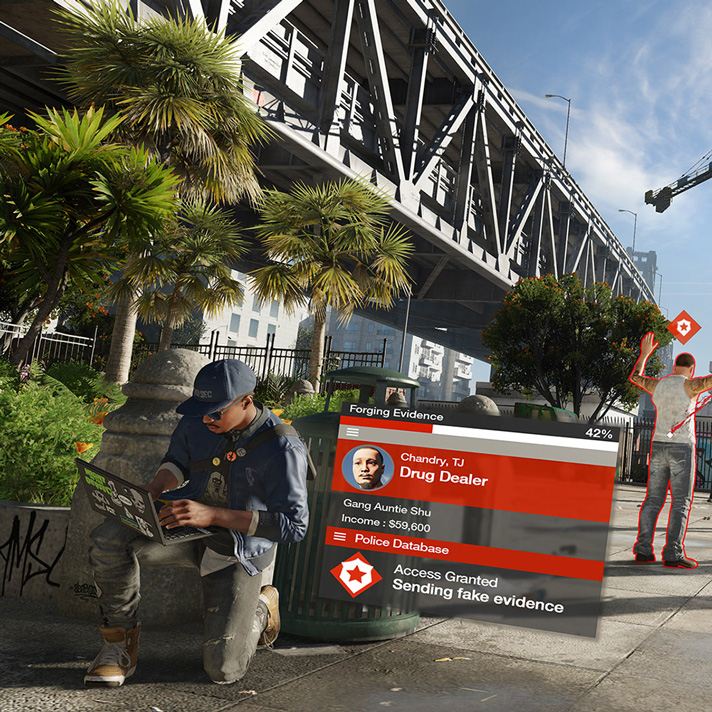
\includegraphics[width=\textwidth]{watch_dogs_2}
		\end{column}
		\pause
		\begin{column}{0.48\textwidth}
			
\includegraphics[height=\textheight]{watch_dogs_2_eula}
		\end{column}
	\end{columns}
\end{frame}

\begin{frame}{Ethical considerations}
	\begin{itemize}
		\pause\item Are you breaching your players' \textbf{privacy}?
		\pause\item Is it right to \textbf{experiment} on your players?
		\pause\item Is it right to \textbf{manipulate} your players' behaviour?
		\pause\item Are you deliberately adding \textbf{addictive} qualities to your game?
		\pause\item Is the above justified if it improves the player \textbf{experience}?
		\pause\item What if it improves your \textbf{profits} instead / as well?
	\end{itemize}
\end{frame}

\begin{frame}{Legal considerations}
	\begin{itemize}
		\pause\item \textbf{NB: this slide is for education only and does NOT constitute legal advice!}
        \pause\item Legislation such as the \textbf{General Data Protection Regulation (GDPR)} and the
            \textbf{Data Protection Act}
		\pause\item Covers \textbf{personal data}: any data that can be used to identify a living individual
			\begin{itemize}
				\pause\item Name, phone number, email address, IP address, social media ID, ...
			\end{itemize}
		\pause\item Covers the \textbf{processing} (including storage) of personal data
		\pause\item The data processor has certain \textbf{responsibilities}
		\pause\item The data subject has certain \textbf{rights}
		\pause\item Not complying can be a \textbf{civil and/or criminal offence}
	\end{itemize}
\end{frame}

\part{What is science?}
\frame{\partpage}

{
\setbeamercolor{background canvas}{bg=}
\includepdf[pages=2-]{../Campelo/01-WhatsScience/Chapter01}
}

\part{The role of experimentation}
\frame{\partpage}

{
\setbeamercolor{background canvas}{bg=}
\includepdf[pages=2-]{../Campelo/02-TheRoleOfExperimentation/Chapter02}
}


\begin{frame}
	\frametitle{Next Week}
	\begin{itemize}
		\item \textbf{Locate and read} at least \textbf{TEN} academic papers from your research area (using ACM DL and IEEE eXplore)
		\item \textbf{Search} for potential gaps in the literature which you think your work could fill---try to articulate it explicitly
		\item \textbf{Devise} a research question that strives to be clear and succinct
		\item \textbf{Fork} the IEEE-style document on BitBucket, and email the link to your supervisor
		\item \textbf{Fork} the computing artefact repo on BitBucket, and email the link to your supervisor
		\item \textbf{Prepare} a draft proposal of 250-or-so words to take to the workshop next week, and push it into your repo	
	\end{itemize}
\end{frame}

\end{document}
